\chapter{SIFT}
Алгоритм \textbf{SIFT} був вперше запропонований Ловом\cite{Lowe2004}. З того часу він зазнав багатьох модифікацій та вдосконалень. Метод SIFT дозволяє знаходити набір особливостей зображень, інваріантних відносно позиції, повороту та масштабування, що дозволяє проводити співставлення з великою кількістю еталонних зображень та забезпечує стійкість до широкого спектру афінних спотворень, змін 3D точки зору, змін в рівні шуму, освітленості. Особливості є досить розрідженими, тобто кожна особливість може бути співставлена з високою ймовірністю з великою базою даних особливостей з різних зображень. Обчислювальна складність визначення особливостей зменшена за рахунок використання підходу каскаду фільтрів, в якому найбільш складні операції застосовуються лише для частин зображення, що проходять початкові тести. Отримання набору особливостей конкретного зображення складається з наступних кроків:

\begin{enumerate}

\item \textbf{Визначення екстремумів в масштабно-просторовому представленні}: перша частина обчислень проводить пошук по всім можливим масштабам та позиціям зображення. Ця операція ефективно реалізована за допомогою функції гаусівської різниці для визначення потенційних критичних точок, інваріантно, відносно масштабу та орієнтації.

\item \textbf{Локалізація ключових точок}: в кожній потенційній позиції застосовується детальна модель для визначення позиції та масштабу. Ключові точки вибираються за мірою їх стійкості.

\item \textbf{Визначення орієнтації}: одна, або більше орієнтацій визначається для кожної ключової точки, в залежності від напрямів локальних градієнтів зображення. Усі наступні перетворення виконуються відносно до визначених орієнтації, масштабу та позиції для кожної особливості зображення, надаючи інваріантність відносно цих перетворень.

\item \textbf{Дескриптор ключової точки}: при вибраному масштабі розглядаються локальні градієнти зображення навколо кожної ключової точки. Вони перетворюються до вигляду, що враховує значні локальні спотворення контурів та освітлення.

\end{enumerate}

Цей підхід було названо Інваріантним відносно Масштабу Перетворенням Особливостей (Scale Invariant Features Transform, SIFT), оскільки він перетворює дані зображення в маcштабо-незалежні координати, відносно локальних особливостей.

\section{Визначення екстремумів в масштабно-просторовому представленні}
\label{sec:sift scale space extrema}

Як було зазначено вище, першим етапом роботи вказаного алгоритму є визначення положення та масштабу точок, що будуть досліджуватись на наступних етапах. Для цього необхідно знайти ключові особливості зображення, що є стійкими до зміни масштабу та орієнтації об'єкту. Це досягається пошуком по всіх можливих масштабах, використовуючи неперервну функцію для зменшення масштабу~\cite{Witkin83}. 

Кьондерінком~\cite{Koenderink84} та Ліндебергом~\cite{Lindeberg94scale-spacetheory} було показано, що за умов деяких очевидних припущень, єдиним допустимим масштабно-просторовим ядром є гаусівська функція, тому масштабно-просторовим виглядом зображення є функція $L(x, y, \sigma)$, отримана в результаті згортки гаусівської функції змінного масштабу $G(x,y,\sigma)$ з вихідним зображенням $I(x,y)$:

\[
L(x,y,\sigma) = G(x,y,\sigma) \ast I(x,y)
\]

де $\ast$ - оператор згортки по $x$ та $y$, а

\[
  G(x,y,\sigma) = \frac{1}{2\pi\sigma^2}e^{-(x^2+y^2)/2\sigma^2}.
\]

Для ефективного визначення стійких ключових точок було запропоновано~\cite{Lowe99objectrec} використовувати масштабно-просторові екстремуми згортки різниці гаусівських функцій з зображенням $D(x,y,\sigma)$, що отримано з різниці двох сусідніх масштабів, що відрізняються сталим коефіцієнтом $k$:

\begin{align}
  \label{eq:dog-scale}
    D(x,y,\sigma) & = (G(x,y,k\sigma) - G(x,y,\sigma)) \ast I(x,y) \notag\\
                  & = L(x,y,k\sigma) - L(x,y,\sigma)
\end{align}

\coolfigure{dog}{Схема побудови масштабно-просторової моделі зображення}{fig:dog}

Емпірично було досліджено~\cite{Lowe2004}, що найкращі результати досягаються для $k=\sqrt2$.

Ефективний підхід до побудови $D(x,y,\sigma)$ зображено на рисунку~\ref{fig:dog}. Вихідне зображення поступово згортається з гаусівськими функціями для отримання зображень з масштабного простору, що відрізняються масштабом в $k$ разів (зліва). Далі, кожна октава масштабного простору (тобто проміжок, границі якого відрізняються вдвічі) ділиться на $s$ інтервалів, тоді $k = 2^{1/s}$. Після цього, з використанням гаусівського фільтра, ми отримуємо $s+3$ зображення для першої октави. З них ми отримаємо значення $D(x,y,\sigma)$ для $s+2$ масштабів: на $s$ шукатимемо екстремум та $2$ --- для граничних умов. Далі, зображення наступної октави можемо отримати, вибравши кожний другий піксель з відповідного зображення попередньої октави.

\coolwfigure{ss_extr}{Кожна точка вибірки порівнюється з її 26 сусідами для пошуку локальних екстремумів}{fig:ss-extr}{0.5\linewidth}

Для визначення локальних екстремумів функції $D(x,y,\sigma)$ кожна точка вибірки порівнюється з 8 сусідніми точками на цьому ж зображенні та по 9 сусідів на наступних більшому та меншому масштабі (рис~\ref{fig:ss-extr}).

\section{Уточнення позицій ключових точок}

Точність знаходження екстремумів може бути збільшена, за допомогою використання розкладання в ряд Тейлора до другого порядку~\cite{Brown02invariantfeatures}:

\begin{equation}
  \label{eq:d-taylor}
  D(\mathbf{x}) = D + {\frac{\partial D}{\partial \mathbf{x}}}^T \mathbf{x} + \frac12 \mathbf{x}^T \frac{\partial ^2 D}{\partial\mathbf{x}^2}\mathbf{x}
\end{equation}

Звідки можна оцінити $\hat{\mathbf{x}}$:

\begin{equation}
  \label{eq:extr-est}
  \hat{\mathbf{x}} = -\left(\frac{\partial^2 D}{\partial \mathbf{x}^2}\right)^{-1} \frac{\partial D}{\partial \mathbf{x}}
\end{equation}

де $D$ та всі відповідні похідні визначаються в досліджуваній точці вибірки, а $\mathbf{x} = (x,y,\sigma)^T$. Якщо відхилення в будь-якому напрямку виявляється більшим за $0.5$, то досліджувану точку змінюють сусідньою та проводять уточнення заново. Після визначення $\hat{\mathbf{x}}$, його значення додають до досліджуваної точки вибірки. Це і є знайдена точка локального екстремуму. 

Підставивши (\ref{eq:extr-est}) в (\ref{eq:d-taylor}), отримаємо значення $D(\hat{\mathbf{x}})$:

\begin{equation*}
  D(\hat{\mathbf{x}}) = D + \frac12 {\frac{\partial D}{\partial x}}^T \hat{\mathbf{x}}
\end{equation*}

Що в подальшому може бути використано для відкидання точок з низькою контрастністю.

\section{Визначення орієнтації}

Відшукавши адекватну орієнтацію для кожної ключової точки, базуючись на локальних властивостях зображення, її дескриптор може бути описаним відносно цієї орієнтації, тобто досягнемо інваріантне представлення, відносно повороту зображення.

Для пошуку локальних орієнтацій використовується розмите зображення $L$, що відповідає найближчому масштабу. Це забезпечує інваріантість всіх обчислень відносно масштабування. Для кожної точки, $L(x,y)$, спочатку підраховуються значення довжини градієнту, $m(x,y)$, та орієнтації, $\theta(x,y)$, за допомогою піксельних різниць:

\[
  m(x,y) = \sqrt{(L(x+1, y) - L(x-1, y))^2 + (L(x,y+1) - L(x,y-1))^2} 
\]

\[
  \theta(x,y) = \tan^{-1}((L(x,y+1) - L(x,y-1)) / (L(x+1,y) - L(x-1,y)))
\]

З орієнтацій сусідніх точок створюють гістограму орієнтацій. Для цього вибирають точки з квадрату $16\times16$~\cite{Meng_implementingthe} навколо досліджуваної, та складають з них гістограму, попередньо зваживши їх значення довжиною градієнта та гаусівським вікном з $\sigma$, що в 1.5 перевищує поточний масштаб ключової точки. Кількість елементів гістограми обмежують 36-ма, що покриває всю $360^\circ$ область можливих напрямів.

Піки на гістограмі орієнтацій відповідають домінантним напрямам локальних градієнтів. Для наступних обчислень використовують найбільший пік та напрями, значення яких вище за 80\% найвищого піку. Кожен з обчислених піків інтерполюють за допомогою параболи через 3 сусідні значення. В подальшому кожній з отриманих орієнтацій ставиться у відповідність окремі ключові точки з однаковою позицією на площині зображення та в масштабному просторі. 

\begin{figure}[h]
  \begin{minipage}[h]{0.49\linewidth}
    \center{\includegraphics[width=0.5\linewidth]{sift-local-gradients} \\
    Довжини і напрямки локальних градієнтів у кожній точці в квадратній області навколо досліджуваної. Вони зважуються гаусівським вікном, що позначене синім колом.
    }
  \end{minipage}
  \hfill
  \begin{minipage}[h]{0.49\linewidth}
    \center{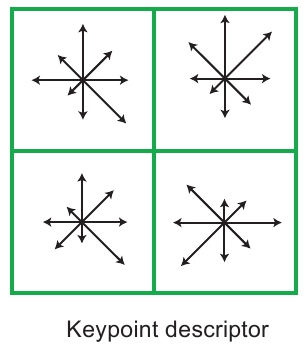
\includegraphics[width=0.5\linewidth]{sift-keypoint-descriptor} \\
    Значення локальних градієнтів з областей $4\times4$ збираються в гістограми з 8-и елементів. Довжини стрілок відповідають сумі довжин локальних градієнтів, близьких за напрямом, в рамках відповідної області.
    }
  \end{minipage}
  \caption{Побудова SIFT-дескрипторів.}
  \label{fig:sift-descriptor}
\end{figure}

\section{Побудова дескрипторів}

Задачею цього етапу є побудова дескрипторів, що максимально відрізняли б кожну ключову точку. Для цього використовуються довжини та напрями градієнтів навколо досліджуваної ключової точки. Ці значення зображені у вигляді маленьких стрілок у відповідних клітинках на рис~\ref{fig:sift-descriptor}.

На правій частині рис.~\ref{fig:sift-descriptor} зображено отриманий дескриптор ключової точки. На рисунку зображено масив $2\times2$ гістограм орієнтації в той час, як на практиці раціонально використовувати масиви розміром $4\times4$ з 8 значеннями орієнтацій в кожному. Тоді кожній ключовій точці буде відповідати вектор з $4\times4\times8=128$ координатами. 

Кінцевим кроком можна нормалізувати вектори до одиничної довжини, що зменшить вплив зміни контрастності зображення.

Після отримання дескрипторів для всіх ключових точок кожного з досліджуваних зображень, перевірити наявність об'єктів з одних зображень на інших можна за допомогою порівняння (наприклад в евклідовій метриці) значень векторів ключових особливостей кожного із зображень. 

Приклад порівняння двох зображень приведено на рис.~\ref{fig:sift-sample}.

\begin{figure}[h]
  \begin{minipage}[h]{0.49\linewidth}
    \center{
    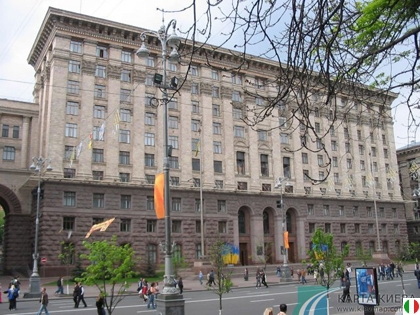
\includegraphics[width=\linewidth]{meria-vhod} \\
    \includegraphics[width=\linewidth]{meria-arka} \\
    }
  \end{minipage}
  \hfill
  \begin{minipage}[h]{0.49\linewidth}
    \center{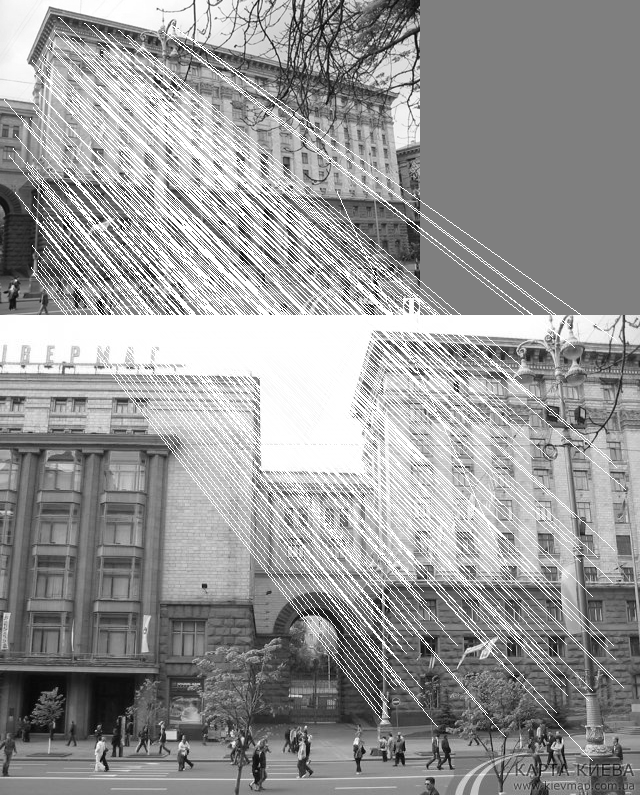
\includegraphics[width=\linewidth]{sift-out} \\
    }
  \end{minipage}
  %\caption{Побудова SIFT-дескрипторів}
  \label{fig:sift-sample}
  \caption{Приклад порівняння зображень за допомогою SIFT.}
\end{figure}
